\documentclass[12pt]{article}
\usepackage{siunitx} % Fornece suporte para a tipografia de unidades do Sistema Internacional e formatação de números
\usepackage{booktabs} % Melhora a qualidade das tabelas
\usepackage{tabularx} % Permite tabelas com larguras de colunas ajustáveis
\usepackage{graphicx} % Suporte para inclusão de imagens
\usepackage{ragged2e} % Justificação de texto melhorada
\usepackage{setspace} % Controle do espaçamento entre linhas
\usepackage[a4paper, left=3.0cm, top=3.0cm, bottom=2.0cm, rigH=2.0cm]{geometry} % Personalização das margens do documento
\usepackage{lipsum} % Geração de texto dummy 'Lorem Ipsum'
\usepackage{fancyhdr} % Customização de cabeçalhos e rodapés
\usepackage{titlesec} % Personalização dos títulos de seções
\usepackage[portuguese]{babel} % Adaptação para o português (nomes e hifenização)
\usepackage{hyperref} % Suporte a hiperlinks
\usepackage{indentfirst} % Indentação do primeiro parágrafo das seções
\usepackage{siunitx} % (Este pacote está duplicado, você pode querer removê-lo)
\usepackage{amsmath}  % Necessário para o ambiente cases
\usepackage{float}
\usepackage{microtype}
\sisetup{
  output-decimal-marker = {,},
  inter-unit-product = \ensuremath{{}\cdot{}},
  per-mode = symbol
}
\DeclareSIUnit{\real}{R\$}
\newcommand{\real}[1]{R\$#1}
\usepackage{float} % Melhor controle sobre o posicionamento de figuras e tabelas
\usepackage{footnotehyper} % Notas de rodapé clicáveis em combinação com hyperref
\usepackage{hyperref} % (Este pacote está duplicado, você pode querer ajustar isso)
\hypersetup{
    colorlinks=true,
    linkcolor=black,
    filecolor=magenta,      
    urlcolor=cyan,
    pdfborder={0 0 0},
}
\usepackage[normalem]{ulem} % Permite o uso de diferentes tipos de sublinhados sem alterar o \emph{}
\makeatletter
\def\@pdfborder{0 0 0} % Remove a borda dos links
\def\@pdfborderstyle{/S/U/W 1} % Estilo da borda dos links
\makeatother
\onehalfspacing

\begin{document}

\begin{titlepage}
    \centering
    \vspace*{1cm}
    \Large\textbf{Insper - Instituto de Ensino e Pesquisa}\\
    \vspace{1.5cm}
    \Large\textbf{Atividade Prática Superviosionada I}\\
    \textbf{Microeconomia IV}\\
    \vspace{1.5cm}
    Prof. Adriano Dutra Teixeira e Prof. Luiz Felipe Fontes\\
    Prof. Auxiliar Pedro Picchetti \\
    \vfill
    \normalsize
    Andreas Azambuja Barbisan - \href{mailto:andreasab@al.insper.edu.br}
    {andreasab@al.insper.edu.br}\\
    Bruno Frasão Brasil Leiros - \href{mailto:brunofbl@al.insper.edu.br}{brunofbl@al.insper.edu.br}\\
    Diogo Roecker Cardozo - \href{mailto:diogorc@al.insper.edu.br}
    {diogorc@al.insper.edu.br}\\
    Lorena Liz Giusti e Santos - \href{mailto:lorenalgs@al.insper.edu.br}{lorenalgs@al.insper.edu.br}\\

    5º Período - Economia A - Grupo 8\\
    \vfill
    São Paulo\\
    Setembro/2024
\end{titlepage}

\pagestyle{fancy}
\fancyhf{}
\rhead{\thepage}

\section*{1-A) Premissas dos Modelos}

\begin{enumerate}
    \item Os indivíduos podem optar entre dois tipos de comportamentos para obter renda: comportamentos legais (\emph{l}) e ilegais (\emph{i}). O tempo gasto em comportamentos legais é denotado por $t_{l}$ e em comportamentos ilegais por $t_{i}$.
    
    \item A renda de um indivíduo é função do tempo gasto em comportamentos legais e ilegais. A receita obtida de comportamentos legais é $W_{l}(t_{l})$ e de comportamentos ilegais é $W_{i}(t_{i})$.
    
    \item Assumimos que a renda pessoal pode ser dividida em dois casos para análise, em que H representa o valor presente líquido dos ativos de um indivíduo, ou seja, a riqueza inicial que um indivíduo possui.
\end{enumerate}

Caso A, no qual os indivíduos envolvidos em comportamentos ilegais não
foram punidos:
\[W\textsubscript{A} = H + W_{l}\left( t_{l} \right) + W_{i}(t_{i})\]

Caso B em que os indivíduos envolvidos em comportamentos ilegais foram
punidos:
\[W\textsubscript{B} = H + W_{l}\left( t_{l} \right) + W_{i}\left( t_{i} \right) - F_{i}(t_{i})\]

Nesse caso, por ele ser pego no ato criminoso, há uma punição na receita
total obtida pelo individuo.

  
  \vspace*{1cm}
\textbf{Problema de maximização do criminoso:}

Dada as premissas, o problema de maximização do criminoso envolve a
escolha entre dois tipos de comportamentos para maximizar sua utilidade
esperada, representada pela expressão U = U (\(W_{s}\), \(t_{c}\)):
comportamentos legais e comportamentos ilegais.

Nesta expressão, "s" refere-se aos dois estados possíveis: ser punido
ou não punido, enquanto ``\(t_{c}\)'' representa o tempo dedicado pelo
grupo de indivíduos. Para determinar como o tempo deve ser alocado entre
atividades legais ou ilegais, a função que maximiza a utilidade pessoal
se dá por:

\[Max:EU\left( W_{s},t_{c} \right) = \sum_{}^{}{\pi s\ U(W_{s},t_{c})} = (1 - p)*U\left( W_{a},t_{c} \right) + p*U(W_{b},t_{c})\]

onde $\pi_s$ representa a probabilidade de um grupo de indivíduos
ser punido ou não pelos comportamentos ilegais. O criminoso busca
maximizar sua utilidade esperada ``\emph{EU}'' com base nas rendas
obtidas de comportamentos legais e ilegais, considerando também a
probabilidade de ser punido (p) ou não punido (1 - p) ao realizar
atividades ilegais. Dessa forma, a utilidade geral de um grupo de
indivíduos em dedicar tempo ao crime ou a atividades legais se dá pelo
somatório das utilidades individuais de cada indivíduo entre alocar
tempo em atividades legais e ilegais.

O tempo total disponível é a soma do tempo dedicado a comportamentos
legais "\(t_{l}\)", ilegais "\(t_{i}\)", e ao tempo de consumo de um
grupo de indivíduos ``\(t_{c}\)'':

\[t\  = \ t_{l}\  + \ t_{i}\  + \ t_{c}\]

Independentemente de comportamentos ilegais ou legais, o benefício W é
uma função crescente do tempo t, e o incremento diminui com o tempo:

\[wi = \frac{dW_{i}}{dt_{i}} > 0\]

\[w^{'}i = \left( \frac{dW_{i}}{dt_{i}} \right)^{'}0\]

\[wl = \frac{dW_{l}}{dt_{l}}0\]

\[w^{'}l = (\frac{dW_{l}}{dt_{i}})'0\]

Após resolver o problema de maximização, as condições de primeira ordem
indicam que o criminoso vai escolher entre comportamentos legais e
ilegais com base na relação marginal de utilidade e nas penalidades
associadas:
\[- \frac{W_{i} - W_{l}}{W_{i} - W_{l} - F_{i}} = \frac{pU'(W_{a})}{(1 - p)U'(W_{b})}\]

Se a taxa de retorno de comportamentos ilegais por unidade de tempo for
muito maior do que a de comportamentos legais, então o tempo que os
indivíduos dedicarão a comportamentos ilegais aumentará.


 \vspace*{1cm}
\textbf{Resultado teórico do modelo}

\begin{enumerate}
    \item Se a taxa de retorno de atividades ilegais (\(W_{i}\)) for
significativamente maior que a de atividades legais (\(w_{l}\)), e o
custo de ser punido (\(f_{i}\)) for baixo, o criminoso tende a dedicar
mais tempo a comportamentos ilegais (\(t_{i}\)).
    
    \item Se a diferença entre o retorno das atividades legais e ilegais for
pequena, o criminoso prefere dedicar mais tempo a atividades legais,
reduzindo "\(t_{i}\)".
\end{enumerate}


\begin{center}
\(\frac{\partial wi}{\partial tl} < 0\) ;
\(\frac{\partial wl}{\partial ti} < 0\)
\end{center}

Dessa forma, com o aumento dos preços das habitações (H), a renda real
de comportamentos legais (\(w_{l}\)) diminui, levando potencialmente a
um aumento no tempo gasto em atividades ilegais para compensar a redução
na renda legal. Esta relação é dada por:


\[\frac{\partial wl}{\partial h} < 0\]

Onde a relação entre o tempo gasto em atividades ilegais e o aumento dos
preços das habitações se dá por:

\[\frac{\partial ti}{\partial h} = \ \frac{\partial ti}{\partial wi}*\frac{\partial wi}{\partial tl}*\frac{\partial tl}{\partial wl}*\frac{\partial wl}{\partial h} > 0\]


Dessa forma, o aumento dos preços das habitações pode influenciar a
decisão de alocação de tempo, reduzindo o incentivo para atividades
legais e aumentando o incentivo para atividades ilegais, à medida que a
pressão financeira aumenta.

Por fim, há duas hipóteses econômicas construídas no artigo que convergem para que o aumento dos preços nas habitações na China leva ao aumento da criminalidade. A primeira hipótese sugere que o preço da moradia é uma variável explicativa que influencia as atividades criminosas de forma positiva. O aumento dos preços das casas pode reduzir a renda real disponível para consumo, dessa forma, quando o retorno das atividades legais diminui em relação ao retorno das
atividades ilegais, as pessoas tendem a alocar mais tempo em atividades
ilegais para compensar essa perda. A segunda hipótese aborda o impacto
indireto dos preços das moradias sobre o crime, de forma que, quando os
preços das casas sobem, o valor dos ativos dos proprietários também
aumenta, permitindo que eles consumam mais. Por outro lado, quem não
possui uma casa ou tem menor valor em imóveis vê sua capacidade de
consumo reduzida, gerando desigualdade. Assim, o aumento no preço das
moradias amplia essa desigualdade, o que pode levar ao aumento das
atividades criminosas.


  \vspace*{1cm}
\section*{B) Estratégia de Identificação}

He e Barkowski (2020) empregam a noção de exogeneidade estrita como ferramenta para identificação. Essa condição é atendida quando os erros (ou resíduos) não possuem qualquer correlação com as observações da amostra. Isso implica que a variável explicativa não é influenciada pelos erros ou por choques, e que os erros, por sua vez, não dependem de valores futuros da variável explicativa.

Formalmente, essa relação pode ser expressa como:
\[
E(u_t | X_1, X_2, \dots, X_T) = 0
\]

Em outras palavras, a esperança condicional dos erros $u_t$ é igual a zero, dado que são condicionados às observações de $X$, independentemente dos períodos de observação.


 \vspace*{1cm}
\textbf{Racional para as Tabelas e Gráficos}

O racional do artigo é de que a Expansão do \emph{Medicaid} aumentaria o
custo de oportunidade dos agentes para cometer um crime e dessa forma
diminuiria a taxa de criminalidade. Os gráficos e tabelas demonstram os
resultados dos testes empíricos realizados pelos autores para dar
suporte a hipótese levantada.


\vspace*{1cm}
\textbf{Interpretação de Resultados}

Tabela 2: Dispõe as estatísticas descritivas Média e Desvio Padrão para
os grupos: Todos os Estados Fronteiriços, Estados que tiveram expansão e
Estados que não tiveram expansão do \emph{Medicaid.}\\


Tabela 3: Dispõe as estatísticas descritivas Média e Desvio Padrão para
os grupos: Todos os Condados Fronteiriços, Condados que tiveram expansão
e Condados que não tiveram expansão do \emph{Medicaid.}\\


Tabela 4: Dispõe os dados estimados pelo método \emph{Diff-in-Diff} do
efeito do \emph{Medicaid} nas taxas de criminalidade por 100.000
habitantes. Todos os valores estimados são negativos indicando uma
relação negativa entre os subgrupos de criminalidade e a expansão do
programa de saúde americano.\\


Tabela 5: Apresenta os dados de robustez para averiguar os dados
dispostos na tabela 4. Foi retirado os estados que já tinham expansões
do \emph{Medicaid} prévias a 2014 mas ainda assim o efeito permaneceu
negativo e significante, como também, foi incluído tendencias temporais
especificas de cada estado mas os efeitos permaneceram robustos.\\


Tabela 6: Estima o ganho de bem-estar gerado pela redução dos crimes nos
estados que expandiram o \emph{Medicaid.} O bem-estar gerado foi
calculado pela perda de bem-estar, crimes totais em expansão e
porcentagem estimada da redução da criminalidade, a multiplicação entre
os três fatores resulta no ganho implícito anual de bem-estar. Foi
estimado um ganho de US\$ 10,5 Bilhões.\\


Gráfico 1: Demonstra que o efeito do \emph{Medicaid} para crimes contra
a propriedade e crimes violentos foi negativo, ou seja, a expansão do
programa de saúde diminuiu as taxas de criminalidade no nível de estado.\\


Gráfico 2: Demonstra o impacto do \emph{Medicaid} para cada subcategoria
de crime: Roubo, Homicídio Doloso, Arrombamento, Furto, Furto de Veículo
e Agressão para os estados americanos. Em todas as subcategorias houve
um impacto negativo do \emph{Medicaid} na taxa de crime para cada
100.000 habitantes.\\


Gráfico 3: Demonstra que o efeito do \emph{Medicaid} para crimes contra
a propriedade e crimes violentos foi negativo, ou seja, a expansão do
programa de saúde diminuiu as taxas de criminalidade no nível de
condado.\\


Gráfico 4: Demonstra o impacto do \emph{Medicaid} para cada subcategoria
de crime: Roubo, Homicídio Doloso, Arrombamento, Furto, Furto de Veículo
e Agressão para os condados americanos. Em todas as subcategorias houve
um impacto negativo do \emph{Medicaid} na taxa de crime para cada
100.000 habitantes.\\



\vspace*{1cm}
\textbf{Principal Resultado do Artigo}

O principal resultado do artigo sugere que a política analisada teve um
impacto significativo e positivo sobre a variável de interesse. A
robustez dos resultados através de várias especificações de modelos e
análises de subgrupos reforça a validade das conclusões.


\vspace*{1cm}
\textbf{Possível Ameaça à Identificação}

Há algumas possíveis ameaças a estratégia adotada por He \& Barkowski,
entre as quais:
\begin{enumerate}
    \item \textbf{Tendências diferentes ao longo do tempo}, para garantir que faça
sentido a análise é necessário que as tendencias de criminalidade entre
os estados que expandiram o \emph{Medicaid} e os que não tenham evoluído
de forma igualitária, caso houvesse alguma assimetria nesse sentido, a
estimação estaria superestimando ou subestimando o impacto do
\emph{Medicaid.}
    
    \item \textbf{Mudanças na legislação e/ou na política,} caso os estados
analisados tenham adotado ou abandonado alguma legislação sobre
segurança pública que tenha tido impacto na criminalidade durante o
período de análise pode estar novamente tendo problemas na estimação do
modelo proposto no artigo.

\end{enumerate}
\vspace*{1cm}
\section*{2-A)}


Nos últimos anos, diversos estados nos Estados Unidos aprovaram leis que
garantem o direito dos cidadãos ao porte de armas de fogo, conhecidas
como leis \emph{shall-issue} ou \emph{Right-to-Carry (RTC)}. A pesquisa
na vertente da Economia do Crime, com base nos bancos de dados
sugeridos, visa identificar possíveis mudanças nas séries históricas
antes e após a implementação dessas leis, especificamente nos crimes
contra a propriedade. Assim, a questão central que o grupo se propõe a
investigar é: \uline{a implementação da \emph{RTC law} influencia na
diminuição sobre a taxa de crimes contra a propriedade?}

    \vspace*{1cm}

\section*{B)}


Baseado no modelo de Becker (1968) de "Crime e Punição", podemos
criar um modelo de utilidade para um indivíduo que decide se vai cometer
um crime contra a propriedade, levando em consideração a renda legal, a
possibilidade de ser pego pela polícia ou pela vítima armada, e as
perdas associadas a essas situações.\\

\textbf{Variáveis principais:}

1. W: Renda legal ou base do criminoso (o quanto ele ganha com
atividades legais).

2. G: Ganho esperado do crime, que pode ser o valor roubado ao invadir
uma casa.

3. p\textsubscript{pol}: Probabilidade de ser pego pela polícia.

4. p\textsubscript{vit}: Probabilidade de a vítima armada reagir (essa
probabilidade está associada ao fato de a vítima possuir uma arma pelo
programa RTC e ser capaz de usá-la contra o criminoso).

5. q\textsubscript{RTC}: Probabilidade de a vítima estar armada devido à
implementação da lei \emph{Right-to-Carry}..

6. L\textsubscript{pol}: Perda sofrida ao ser pego pela polícia, como
prisão ou multa.

7. L\textsubscript{vit}: Perda sofrida ao ser ferido ou morto pela
vítima armada, ou seja, o custo da reação da vítima.
\newpage
\textbf{Função de Utilidade:}

A utilidade total esperada do criminoso ao cometer um crime pode ser
modelada como a soma da renda legal (W) e do ganho esperado do crime
(G), levando em consideração as probabilidades de ser pego pela polícia
ou ser enfrentado por uma vítima armada.

\begin{align*}
UE &= U(W) + \left( \left( 1 - p_{pol} - (p_{vit} * q_{RTC}) \right) * U(G) \right) \\
   &\quad - \left( p_{pol} * U(L_{pol}) \right) - \left( p_{vit} * q_{RTC} * U(L_{vit}) \right)
\end{align*}

Dessa forma, a função utilidade de não cometer o crime é simplesmente a
renda legal do criminoso, visto que as probabilidades associadas a ele
ser pego é 0 e a utilidade do ganho do roubo (U(G)) também é 0:

\begin{align*}
UE &= U(W) + \left( (1 - 0 - 0) * 0 \right) \\
   &\quad - \left( 0 * U(L_{pol}) \right) - \left( 0 * U(L_{vit}) \right) \\
UE &= U(W)
\end{align*}\\

\textbf{Condição para decisão de cometer o crime:}

O indivíduo decide cometer o crime se a utilidade esperada de cometer o
crime for maior que a utilidade de não o cometer:

\[
UE > U(W)
\]

Substituindo as funções de utilidade:

\begin{align*}
U(W) &+ \left( \left( 1 - p_{pol} - (p_{vit} * q_{RTC}) \right) * U(G) \right) \\
     &\quad - \left( p_{pol} * U(L_{pol}) \right) - \left( p_{vit} * q_{RTC} * U(L_{vit}) \right) > U(W)
\end{align*}

Simplificando a equação:

\begin{align*}
\left( 1 - p_{pol} - (p_{vit} * q_{RTC}) \right) * U(G) &> p_{pol} * U(L_{pol}) \\
                                                         &\quad + p_{vit} * q_{RTC} * U(L_{vit})
\end{align*}

Assim, o lado esquerdo da equação representa o benefício esperado do
crime, considerando que o criminoso não seja pego nem pela polícia nem
pela vítima armada. Já o lado direito representa os custos esperados do
crime, levando em conta a probabilidade de ser pego pela polícia ou de
ser confrontado pela vítima armada.


O criminoso cometerá o crime se o benefício esperado for maior que o
custo esperado. Quanto maior for a probabilidade de ser pego pela
polícia ou a probabilidade de ser confrontado pela vítima armada,
menores as chances de o criminoso decidir cometer o crime. Derivando,
tem-se:
\begin{alignat*}{2}
\frac{\partial UE}{\partial p_{pol}} &= -U(G) - U\left( L_{pol} \right) < 0 \quad &\frac{\partial UE}{\partial p_{vit}} &= -q_{RTC} \cdot (U(G) + U\left( L_{vit} \right)) < 0 \\
\frac{\partial UE}{\partial L_{pol}} &= -p_{pol} < 0 \quad &\frac{\partial UE}{\partial L_{vit}} &= -p_{vit} < 0
\end{alignat*}

A derivada negativa significa que, à medida que a probabilidade de ser
pego pela polícia ou pela vítima aumenta - igualmente se as punições
aumentarem - a utilidade esperada do criminoso diminui.

"G" é o ganho esperado do crime, e "L\textsubscript{pol}" e "L\textsubscript{vit}" é o custo de
ser pego. Ambos contribuem para reduzir a atratividade do crime. Quanto
maior a chance de ser capturado (ppol ou pvit), maior será a perda total
de utilidade. Da mesma forma, quanto maior for o q\textsubscript{RTC}
(probabilidade de a vítima estar armada devido ao RTC), maior será o
impacto negativo na utilidade esperada do criminoso à medida que aumenta
a probabilidade de a vítima estar armada.

\[\frac{\partial UE}{\partial q_{RTC}} = - p_{vit} \cdot \left( U(G) + U\left( L_{vit} \right) \right) < 0\]

Há de se notar que "p\textsubscript{vit}" determina o quão relevante será o
efeito da implementação da RTC sobre a utilidade do criminoso. Quanto
maior for a chance de confronto (p\textsubscript{vit}), maior será a diminuição na
utilidade esperada do criminoso conforme aumenta a probabilidade de a
vítima estar armada (q\textsubscript{RTC}).

Também, quanto maiores forem o custo da punição policial ou o risco de
ser ferido ou morto pela vítima, menor será o incentivo para o crime:

\[\frac{\partial UE}{\partial G} = 1 - p_{pol} - p_{vit} > 0\]

A derivada positiva mostra que quanto maior o ganho esperado do crime,
maior será a utilidade esperada do criminoso. No entanto, esse ganho é
reduzido pelas probabilidades de ser pego pela polícia e pela vítima, de
forma que, quanto maiores essas probabilidades, menor será o impacto
positivo de um maior ganho.

Dessa forma, fundamentado pelo modelo clássico de crime de Becker, a
hipótese econômica do grupo é de que um aumento nos riscos associados ao
crime, como a probabilidade de ser confrontado por uma vítima armada
(probabilidade essa aumentada pelo RTC) ou capturado pela polícia,
resulta em uma redução na quantidade de crimes cometidos em
propriedades.\\


\section*{C) Estatístitcas descritivas}


\begin{figure}[H]
    \centering
    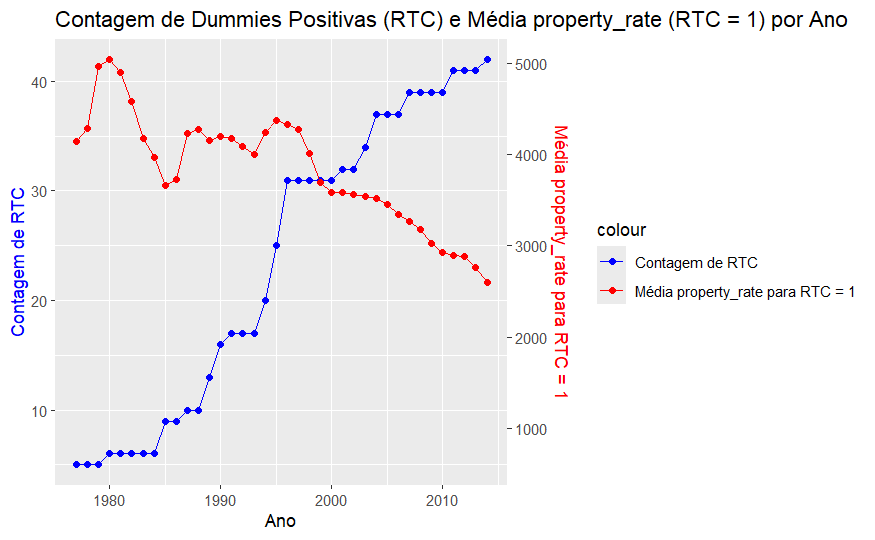
\includegraphics[width=1\linewidth]{grafico1final.png}
    \caption{Fonte: Elaboração Própria}
    \label{fig:enter-label}
\end{figure}




\textbf{Contagem de RTC (linha azul):}

Representa o número de estados dos EUA que passaram a permitir o porte
de armas ao longo do tempo. Vemos um crescimento constante,
especialmente após 1990, quando mais estados começaram a adotar essas
permissões. Antes de 1990, poucos estados tinham essa legislação, mas a
partir desse ponto, houve um aumento significativo, atingindo mais de 40
estados em 2010.

\textbf{Média property\_rate (linha vermelha):}

Representa a taxa média de crimes contra a propriedade nos estados com
permissão para porte de armas. Observa-se que, à medida que mais estados
permitem o porte de armas (crescimento do RTC), a taxa de crimes contra
a propriedade tende a diminuir. No início do gráfico, por volta de 1970,
a taxa era alta (acima de 4000 crimes por 100.000 habitantes, por
exemplo), mas conforme mais estados passaram a adotar RTC, essa taxa foi
caindo significativamente, especialmente após 2000, chegando a menos de
3000 crimes.

\textbf{Interpretação geral:}

A relação entre o número de estados que permitem o porte de armas e a
taxa de crimes contra a propriedade parece ser inversa. Conforme mais
estados passam a permitir o porte de armas (RTC), a taxa de crimes
contra a propriedade tende a diminuir. Isso pode sugerir uma correlação
em que a permissão para o porte de armas impacta a diminuição de crimes
contra a propriedade, embora seja necessário mais contexto ou análise
estatística para confirmar essa relação causal.

\begin{figure}[H]
    \centering
    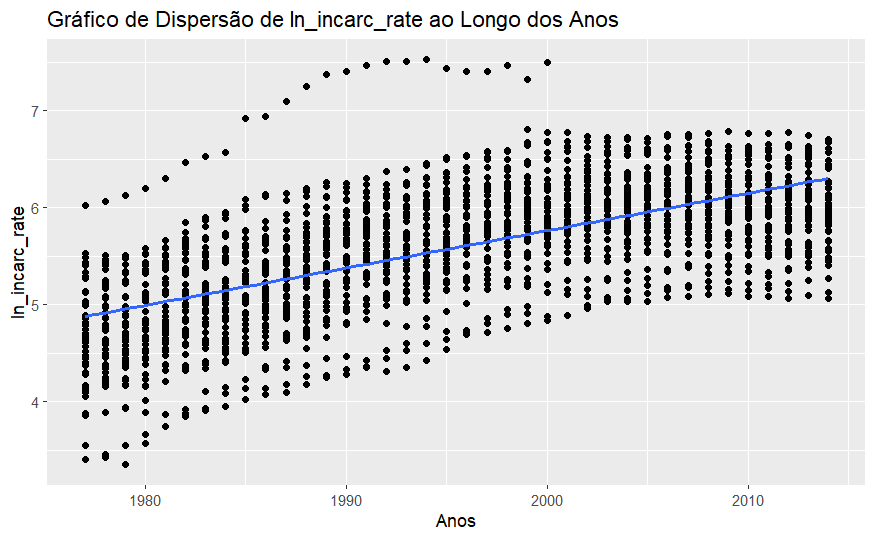
\includegraphics[width=1\linewidth]{grafico2final.png}
    \caption{Fonte: Elaboração Própria}
    \label{fig:enter-label}
\end{figure}

\textbf{Gráfico 2:} Demonstra o Log da taxa de encarceramento ao longo
dos anos.

\textbf{Dispersão dos pontos:}

Observa-se uma grande variação na taxa de encarceramento entre os
estados ao longo do tempo. Contudo, existe uma tendência clara de
aumento. A partir dos anos 1970, os pontos estão mais concentrados em
valores mais baixos, enquanto, ao longo do tempo, essa concentração se
desloca para valores mais altos. Isso indica que as taxas de
encarceramento têm aumentado em muitos estados.

\textbf{Linha de tendência (linha azul):}

A linha de tendência azul mostra um aumento na taxa de encarceramento ao
longo do tempo. Esse aumento é particularmente notável após a década de
1980 e continua a crescer até o final do período analisado.

\begin{figure}[H]
    \centering
    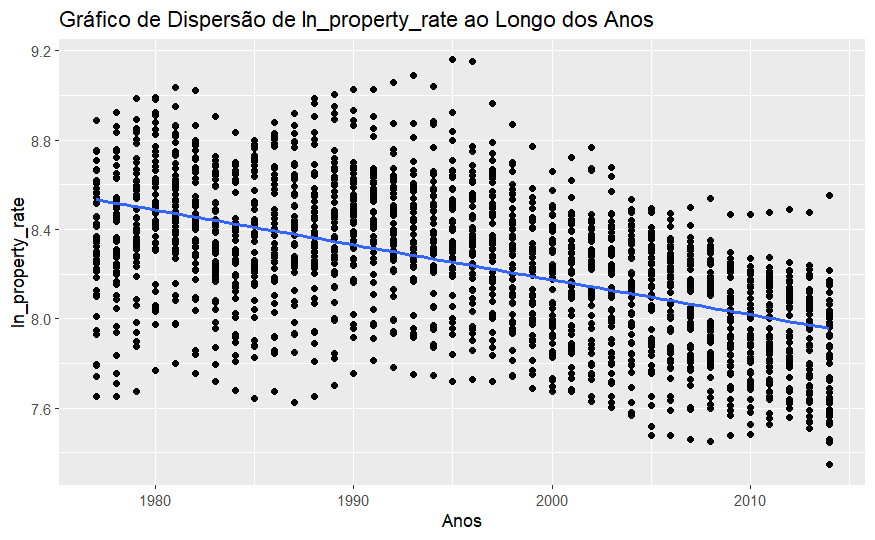
\includegraphics[width=1\linewidth]{grafico3final.png}
    \caption{Fonte: Elaboração Própria}
    \label{fig:enter-label}
\end{figure}

\textbf{Gráfico 3:} Demonstra o Log da quantidade de crimes contra a
propriedade.

\textbf{Dispersão dos pontos:}

A dispersão dos pontos mostra que a taxa de crimes contra a propriedade
variou consideravelmente entre os estados ao longo do tempo. No entanto,
observa-se uma tendência de queda nos valores conforme o tempo avança,
sugerindo que, em geral, os crimes contra a propriedade diminuíram ao
longo das décadas.

\textbf{Linha de tendência (linha azul):}

A linha de tendência azul mostra uma clara diminuição na taxa de crimes
contra a propriedade ao longo do tempo. Isso indica que, em média, os
crimes contra a propriedade nos estados dos EUA caíram de forma
constante de 1970 até 2010. Indicando uma possível influência da maior
implementação do RTC.

\begin{figure}[H]
    \centering
    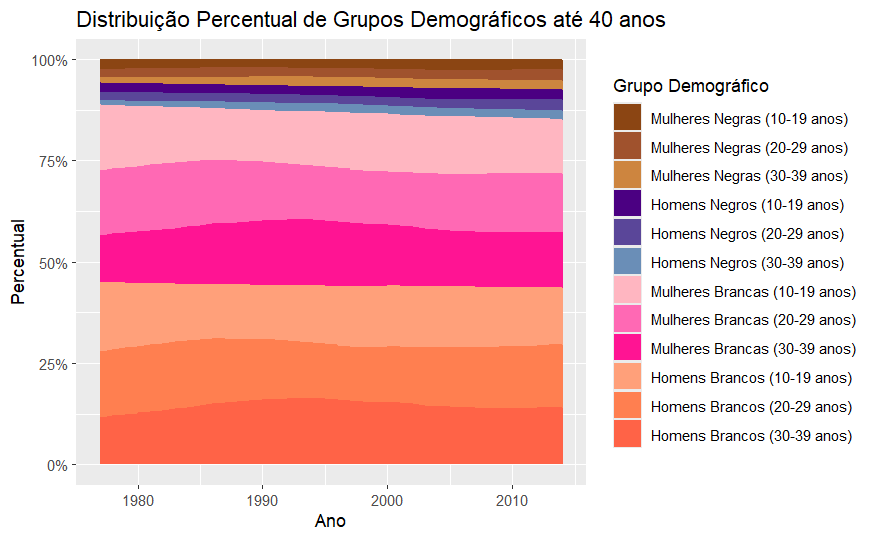
\includegraphics[width=1\linewidth]{grafico4final.png}
    \caption{Fonte: Elaboração Própria}
    \label{fig:enter-label}
\end{figure}

\textbf{Gráfico 4:} Demonstra o percentual que cada grupo demográfico,
de até 40 anos de idade, compõe de toda a população de até 40 anos. É
possível identificar o crescimento do percentual população negra de até
40 anos ao longo dos 30 anos ao passo em que há uma queda do percentual
de homens e mulheres da cor branca de 10 a 19 anos de idade. Em síntese,
há um ligeiro aumento da diversidade racial entre 1980 até 2010.

\begin{figure}[H]
    \centering
    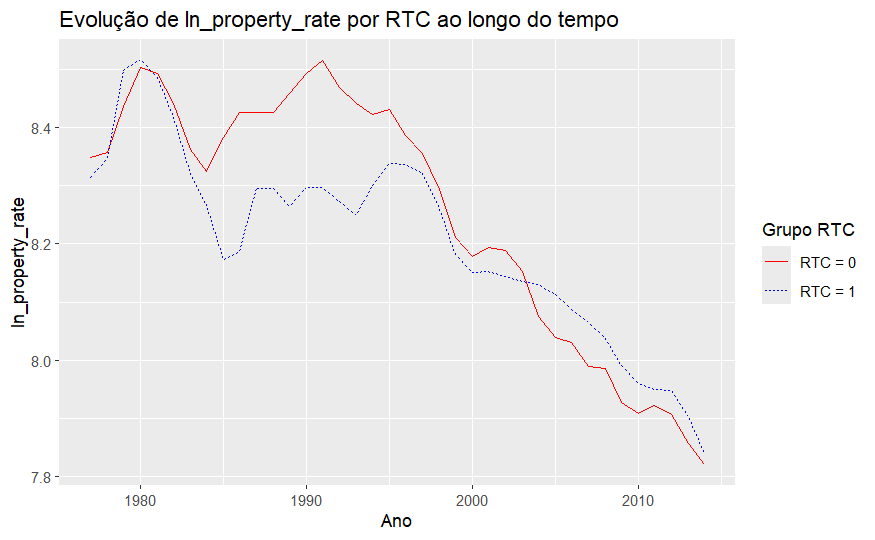
\includegraphics[width=1\linewidth]{grafico5final.png}
    \caption{Fonte: Elaboração Própria}
    \label{fig:enter-label}
\end{figure}

\textbf{Gráfico 5:} Demonstra a evolução do Log da quantidade de crimes
contra a propriedade para tanto os estados que têm o right-to-carry
(linha azul) e estados que não tem (linha vermelha), ao longo dos anos.

É possível perceber que ambas as linhas tem uma tendencia negativa,
porém, durante um período na década de 80, os estados que não tinham RTC
tinham uma criminalidade menor do que os que não tinham. A partir de
meados da década de 90 as linhas se convergem e seguem valores muito
próximos, inclusive com a linha de RTC=1 superando a de RTC=0, no final
da série. Isso indica que talvez a maior implementação do RTC tenha tido
efeito no começo, mas com o passar do tempo pode ser que ter RTC não
faça diferença nos crimes contra a propriedade.

Traçando um paralelo com o primeiro gráfico analisado, provavelmente a
queda na quantidade de crimes contra propriedade não foi causada pelo
aumento do RTC, mas por algum motivo, que também afeta estados sem o RTC


\section*{D)}

A hipótese econômica subjacente ao grupo é que a implementação da RTC
tem o potencial de reduzir a criminalidade, ao diminuir a utilidade
esperada do criminoso. Isso ocorre porque o RTC aumenta a probabilidade
de retaliação por parte da vítima, tornando o crime menos atraente. Para
testar essa hipótese, foram realizados três tipos de regressões:
\emph{Pooled OLS}, Efeitos Fixos e Efeitos Aleatórios. As variáveis
explicativas selecionadas foram a implementação do RTC em cada estado,
índices de criminalidade e fatores demográficos, como raça, gênero e
idade.

A inclusão da variável RTC como explicativa é justificada por ser o foco
central da nossa análise. Estamos interessados em determinar se a adoção
do RTC está associada a uma diminuição nas taxas de criminalidade.
Portanto, essa variável é essencial para testar diretamente a nossa
hipótese

As variáveis relacionadas à criminalidade (como a taxa de
encarceramento, taxa de crimes violentos, taxa de homicídios com e sem
armas de fogo) foram incluídas por serem correlacionadas com a taxa de
crimes contra a propriedade, nossa variável dependente. Elas ajudam a
capturar aspectos importantes do ambiente de segurança pública e
controlam por potenciais fatores de confusão. Além disso, sua inclusão
minimiza problemas de endogeneidade, que poderiam surgir caso essas
variáveis fossem omitidas, levando a estimativas viesadas.

Por fim, os controles demográficos relacionados à raça, gênero e idade
são justificados pela literatura criminológica, que aponta que certos
grupos são mais vulneráveis à criminalidade, tanto como vítimas quanto
como autores de crimes. Fatores como a idade jovem, gênero masculino e
determinados grupos raciais tendem a estar mais fortemente associados ao
envolvimento com crimes, seja como vítimas ou perpetradores. A omissão
dessas variáveis poderia gerar viés nas estimativas, uma vez que esses
fatores influenciam diretamente as taxas de criminalidade. Portanto, o
controle por essas variáveis é essencial para isolar o efeito do RTC e
evitar atribuir a ele efeitos que poderiam estar relacionados a
variações demográficas.

\begin{table}[!htbp] \centering 
  \caption{} 
  \label{} 
  \resizebox{\textwidth}{!}{  % Ajusta a tabela à largura da página
  \begin{tabular}{@{\extracolsep{5pt}}lccc} 
  \\[-1.8ex]\hline 
  \hline \\[-1.8ex] 
   & \multicolumn{3}{c}{\textit{Dependent variable:}} \\ 
  \cline{2-4} 
  \\[-1.8ex] & \multicolumn{3}{c}{ln\_property\_rate} \\ 
   & POLS & FE & RE \\ 
  \\[-1.8ex] & (1) & (2) & (3)\\ 
  \hline \\[-1.8ex] 
   RTC & 0.100$^{***}$ & 0.075$^{***}$ & 0.070$^{***}$ \\ 
    & (0.010) & (0.008) & (0.008) \\ 
    & & & \\ 
   ln\_incarc\_rate & 0.090$^{***}$ & $-$0.071$^{***}$ & $-$0.073$^{***}$ \\ 
    & (0.014) & (0.015) & (0.012) \\ 
    & & & \\ 
   ln\_violent\_rate & 0.298$^{***}$ & 0.336$^{***}$ & 0.346$^{***}$ \\ 
    & (0.014) & (0.015) & (0.014) \\ 
    & & & \\ 
   ln\_DeathsHomi\_rate & $-$0.278$^{***}$ & $-$0.049 & $-$0.034 \\ 
    & (0.092) & (0.057) & (0.049) \\ 
    & & & \\ 
   ln\_DeathsHomi\_fire\_rate & 0.110$^{**}$ & 0.058$^{*}$ & 0.059$^{*}$ \\ 
    & (0.055) & (0.034) & (0.030) \\ 
    & & & \\ 
   ln\_DeathsHomi\_nonfire\_rate & 0.171$^{***}$ & 0.103$^{***}$ & 0.119$^{***}$ \\ 
    & (0.039) & (0.023) & (0.018) \\ 
    & & & \\ 
   age\_bm\_1019 & $-$0.119$^{***}$ & $-$0.140$^{***}$ & $-$0.056$^{***}$ \\ 
    & (0.019) & (0.021) & (0.018) \\ 
    & & & \\ 
   age\_bm\_2029 & 0.008 & 0.032 & $-$0.020 \\ 
    & (0.035) & (0.024) & (0.023) \\ 
    & & & \\ 
   age\_bm\_3039 & 0.061$^{**}$ & 0.077$^{***}$ & 0.160$^{***}$ \\ 
    & (0.027) & (0.026) & (0.021) \\ 
    & & & \\ 
   age\_wm\_1019 & $-$0.028$^{***}$ & 0.079$^{***}$ & 0.102$^{***}$ \\ 
    & (0.007) & (0.009) & (0.006) \\ 
    & & & \\ 
   age\_wm\_2029 & 0.041$^{***}$ & 0.019$^{**}$ & 0.023$^{***}$ \\ 
    & (0.009) & (0.008) & (0.005) \\ 
    & & & \\ 
   age\_wm\_3039 & $-$0.032$^{***}$ & 0.066$^{***}$ & 0.073$^{***}$ \\ 
    & (0.008) & (0.007) & (0.004) \\ 
    & & & \\ 
   Constant & 6.670$^{***}$ &  & 5.193$^{***}$ \\ 
    & (0.139) &  & (0.122) \\ 
    & & & \\ 
  \hline \\[-1.8ex] 
  Year FE & Yes & Yes & No \\ 
  State FE & No & Yes & No \\ 
  Hausman Test Chi-Sq &  &  & 83.0445 \\ 
  Hausman Test p-value &  &  & 0.0000 \\ 
  Observations & 1,822 & 1,822 & 1,822 \\ 
  R$^{2}$ & 0.691 & 0.830 & 0.818 \\ 
  Adjusted R$^{2}$ & 0.682 & 0.820 & 0.817 \\ 
  F Statistic & 80.776$^{***}$ (df = 49; 1772) & 171.714$^{***}$ (df = 49; 1722) & 7,295.114$^{***}$ \\ 
  \hline 
  \hline \\[-1.8ex] 
  \textit{Note:}  & \multicolumn{3}{r}{$^{*}$p$<$0.1; $^{**}$p$<$0.05; $^{***}$p$<$0.01} \\ 
  \end{tabular} 
  }  % Fim do \resizebox
\end{table}



\newpage
Em todas as regressões, os resultados encontrados vão na contramão da
hipótese econômica do grupo: o efeito da RTC, na verdade, tem efeito
positivo sobre a criminalidade. Estes, porém, variam em cada um dos
modelos com relação a magnitude do efeito causal: enquanto no efeito
\emph{pooled}, controlado apenas com fatores temporais, o impacto da
implementação da lei causa um aumento esperado de 10,0\% na taxa de
crimes contra a propriedade, \emph{ceteris paribus}. Enquanto isso, no
efeito fixo e no aleatório o efeito encontrado foi menor, com um aumento esperado de
7,5\% e 7,0\%, respectivamente. Isso indica que no primeiro caso, o
efeito causal estava possivelmente sendo superestimado.

Além disso, o grupo também realizou o teste de Hausman, para verificar
qual dos modelos se demonstra mais adequado para analisar e estimar o
efeito causal. O teste de Hausman ajuda a determinar se há correlação
entre as variáveis explicativas e os efeitos individuais. Neles as
hipóteses são:
\[
\begin{cases}
H_{0}: \text{Não há correlação entre os efeitos individuais e as variáveis explicativas.} \\
H_{1}: \text{Existe correlação entre os efeitos individuais e as variáveis explicativas.}
\end{cases}
\]

Se rejeitar a hipótese nula, deve ser usado o modelo de efeitos fixos, e o
de efeito aleatório seria inconsistente. No caso, o p-valor foi de
aproximadamente 0, então com qualquer nível de significância usual
rejeita-se a hipótese nula e deve ser usado um estimador de efeitos
fixos.

Além disso, também foram estimadas regressões dos mesmos três tipos
(\emph{Pooled OLS}, Efeitos Fixos e Efeitos aleatórios) mas considerando
a exclusão das variáveis relacionadas a gênero, idade ou raça. Nessa
categoria, o resultado encontrado foi levemente diferente, com o
\emph{pooled} resultando em um aumento esperado de 9,2\% nos crimes de
propriedade, \emph{ceteris paribus}, enquanto em efeitos fixos e
aleatórios foi estimado um aumento de 8,2\% e 1,2\%, respectivamente.
Porém, nessa estimação o efeito aleatório foi extremamente discrepante,
e não foi estatisticamente relevante para nenhum nível usual de de
significância.

% Table created by stargazer v.5.2.3 by Marek Hlavac, Social Policy Institute. E-mail: marek.hlavac at gmail.com
% Date and time: sex, set 06, 2024 - 20:45:51
\begin{table}[!htbp] \centering 
  \caption{} 
  \label{} 
  \resizebox{\textwidth}{!}{  % Redimensiona a tabela para ajustar à largura da página
  \begin{tabular}{@{\extracolsep{5pt}}lccc} 
  \\[-1.8ex]\hline 
  \hline \\[-1.8ex] 
   & \multicolumn{3}{c}{\textit{Dependent variable:}} \\ 
  \cline{2-4} 
  \\[-1.8ex] & \multicolumn{3}{c}{ln\_property\_rate} \\ 
   & POLS & FE & RE \\ 
  \\[-1.8ex] & (1) & (2) & (3)\\ 
  \hline \\[-1.8ex] 
   RTC & 0.092$^{***}$ & 0.082$^{***}$ & 0.012 \\ 
    & (0.011) & (0.009) & (0.010) \\ 
    & & & \\ 
   ln\_incarc\_rate & 0.078$^{***}$ & $-$0.048$^{***}$ & $-$0.222$^{***}$ \\ 
    & (0.014) & (0.016) & (0.009) \\ 
    & & & \\ 
   ln\_violent\_rate & 0.317$^{***}$ & 0.330$^{***}$ & 0.466$^{***}$ \\ 
    & (0.014) & (0.016) & (0.017) \\ 
    & & & \\ 
   ln\_DeathsHomi\_rate & $-$0.304$^{***}$ & 0.085 & 0.033 \\ 
    & (0.094) & (0.062) & (0.057) \\ 
    & & & \\ 
   ln\_DeathsHomi\_fire\_rate & 0.068 & $-$0.003 & 0.033 \\ 
    & (0.056) & (0.037) & (0.036) \\ 
    & & & \\ 
   ln\_DeathsHomi\_nonfire\_rate & 0.197$^{***}$ & 0.043$^{*}$ & 0.140$^{***}$ \\ 
    & (0.041) & (0.025) & (0.021) \\ 
    & & & \\ 
   Constant & 6.521$^{***}$ &  & 6.514$^{***}$ \\ 
    & (0.119) &  & (0.105) \\ 
    & & & \\ 
  \hline \\[-1.8ex] 
  Year FE & Yes & Yes & No \\ 
  State FE & No & Yes & No \\ 
  Hausman Test Chi-Sq &  &  & 495.8589 \\ 
  Hausman Test p-value &  &  & 0.0000 \\ 
  Observations & 1,822 & 1,822 & 1,822 \\ 
  R$^{2}$ & 0.659 & 0.792 & 0.718 \\ 
  Adjusted R$^{2}$ & 0.651 & 0.781 & 0.717 \\ 
  F Statistic & 79.903$^{***}$ (df = 43; 1778) & 153.481$^{***}$ (df = 43; 1728) & 3,935.655$^{***}$ \\ 
  \hline 
  \hline \\[-1.8ex] 
  \textit{Note:}  & \multicolumn{3}{r}{$^{*}$p$<$0.1; $^{**}$p$<$0.05; $^{***}$p$<$0.01} \\ 
  \end{tabular} 
  }  % Fim do resizebox
\end{table}



\newpage
Portanto, os resultados indicam que a hipótese econômica proposta não
pode ser validada no contexto de crimes contra a propriedade. Embora se
espere que os infratores considerem a possibilidade de reação por parte
das vítimas após a implementação do RTC, isso não parece resultar em uma
redução significativa na incidência desses crimes. Assim, a presença de
um potencial aumento na retaliação armada não demonstrou, neste estudo,
o efeito dissuasivo esperado sobre crimes de propriedade.

\end{document}